\documentclass[12pt]{article}

\usepackage[margin=1.5cm]{geometry}        % For setting margins
\usepackage[spanish,es-tabla]{babel}
\selectlanguage{spanish}
\usepackage{amsmath}                % For Math
\usepackage{fancyhdr}                % For fancy header/footer
\usepackage{graphicx}                % For including figure/image
\usepackage{cancel}                    % To use the slash to cancel out stuff in working out equations
\usepackage{amsfonts}
\usepackage{color}
\usepackage{bbm}
\usepackage{float}
\usepackage{subcaption}
\usepackage{lipsum}
\usepackage{listings}
\usepackage{algorithm,algpseudocode}
\usepackage{hyperref}
\captionsetup{compatibility=false}

%%%%%%%%%%%%%%%%%%%%%%
% Set up fancy header/footer
\pagestyle{fancy}
\fancyhead[LO,L]{Alejandro Uribe}
\fancyhead[CO,C]{Aprendizaje Reforzado - Guía 1: Multi-armed bandits}
\fancyhead[RO,R]{}
\fancyfoot[LO,L]{}
\fancyfoot[CO,C]{\thepage}
\fancyfoot[RO,R]{\today}
\renewcommand{\headrulewidth}{0.4pt}
\renewcommand{\footrulewidth}{0.4pt}

\newlength\tindent
\setlength{\tindent}{\parindent}
\setlength{\parindent}{0pt}
\renewcommand{\indent}{\hspace*{\tindent}}
\DeclareMathOperator*{\argmax}{argmax}
\floatname{algorithm}{Algoritmo}
%%%%%%%%%%%%%%%%%%%%%%

\begin{document}
    \indent\underline{Ejercicio 1}

    Demostrar que, si conociéramos exactamente el valor de cada acción, es decir, si $Q_{t} (a) = E \left[ R_{t} \big| A_{t}=a \right]$, entonces la acción \textit{greedy} $ A_{t} = \argmax_{a}Q_{t}(a) $ es la acción óptima en el sentido de que permite maximizar las recompensas totales.

    \indent\underline{Solución:}

    Sea,\\
    $a$: Acción arbitraria \\
    $A_{t}$: Acción tomada en el tiempo $t$ \\
    $R_{t}$: Recompensa obtenida en el tiempo $t$ \\
    $Q_{t}(a)$: Valor estimado de la acción $a$ en el tiempo $t$ \\
    $q_{*}(a)$: Recompensa esperada dado que se toma la acción $a$ \\
    Acción \textit{greedy}: acción cuyo valor estimado es el mayor de todos los valores estimados de las acciones posibles en el tiempo $t$ \\

    El valor $q_{*}(a)$ de una acción arbitraria $a$ equivale al valor esperado de la recompensa si $a$ es seleccionada.

    \[ q_{*}(a) \doteq \mathbb{E} \left[ R_{t} \big| A_{t}=a \right] \]

    La aplicación del algoritmo \textit{greedy} implica guardar los valores estimados de las acciones en cada iteración, en una estrategia no exploratoria.
    Se calcula $Q_{t}(a)$ como el valor estimado de la acción $a$ en el tiempo $t$, o bien, promediando las recompensas obtenidas, es decir,

    \begin{gather*}
        Q_{t}(a)
        \doteq
        \frac{\text{suma de las recompensas al tomar \textbf{a} antes de \textbf{t}}}
        {\text{veces que se ha tomado \textbf{a} antes de \textbf{t}}}
    \end{gather*}

    Donde $\mathbbm{1}$ denota una variable aleatoria que toma el valor 1 si la acción $a$ fue seleccionada en el tiempo $t$, y 0 en caso contrario\footnotemark.
    \footnotetext{Si el denominador es 0, se define $Q_{t}(a)$ como un valor por defecto, sea 0}
    La estrategia no exploratoria se interpreta matemáticamente como:

    \[
        Q_t(a)= \frac{ \sum_{i=1}^{t-1} R_{i} \cdot \mathbbm{1} }{ \sum_{i=1}^{t-1} \mathbbm{1}_{A_{i}=a}}
    \]

    De la cual se toma el valor máximo del \textit{Q-valor}, es decir

    \[
        A_{t} = argmax_{a}Q_{t}(a)
    \]

    Si se conociera el valor de $q_{*}(a)$, entonces la acción \textit{greedy} será la acción que maximiza el valor esperado de la recompensa, es decir, la acción $a$ tal que $Q_{t}(a) \approx q_{*}(a)$.

    \line(1,0){\textwidth}

    \indent\underline{Ejercicio 2}

    En una selección de acciones tipo $\varepsilon-greedy$ con dos acciones posibles y $\varepsilon=0.1$, ¿Cuál es la probabilidad de seleccionar la acción \textit{greedy}?

    \indent\underline{Solución:}

    En una estrategia de acciones tipo $\varepsilon-greedy$, se selecciona una acción aleatoria con probabilidad $\varepsilon$ y se selecciona la acción \textit{greedy} con probabilidad $1-\varepsilon$.
    Es decir, si $\varepsilon=0.1$, entonces la probabilidad de seleccionar la acción \textit{greedy} es de $1-\varepsilon=0.9$.
    O bien,

    \[P(\text{acción \textit{greedy}}) = 1-\varepsilon = 1 - 0.1 = 0.9\]

    \line(1,0){\textwidth}

    \indent\underline{Ejercicio 3}
    Demostrar que el valor de una acción después de haber sido seleccionada $n-1$ veces, definido como

    \[ Q_{n} = \frac{R_{1} + R_{2} + \ldots + R_{n-1}}{n-1} \]

    puede calcularse incrementalmente con la siguiente fórmula:

    \[ Q_{n+1} = Q_{n} + \frac{1}{n} \left[ R_{n} - Q_{n} \right] \]

    Describa la ventaja de esta fórmula desde un punto de vista computacional.

    \indent\underline{Solución:}

    Sea,\\
    $Q_{n}$: Valor estimado de la acción después de haber sido seleccionada $n-1$ veces \\
    $R_i$: Recompensa obtenida después de la $i$-ésima selección de la acción \\
    $n$: Número de veces que la acción ha sido seleccionada \\

    Dado que $Q_{n}$ es el promedio de las recompensas obtenidas después de haber seleccionado la acción $n-1$ veces, se tiene que

    \[ Q_{n} = \frac{R_{1} + R_{2} + \ldots + R_{n-1}}{n-1} \]

    O bien puede escribirse como

    \[ Q_{n} = \frac{1}{n-1} \sum_{i=1}^{n-1} R_{i} \]

    O su equivalente en términos de $Q_{n+1}$, al sustituir $n$ por $n+1$ en la fórmula anterior

    \[ Q_{n+1} = \frac{1}{n} \sum_{i=1}^{n} R_{i} \]

    Si se desea calcular el valor de la acción después de haber sido seleccionada $n$ veces, se puede hacer de manera incremental, es decir, se puede calcular el valor de la acción después de haber sido seleccionada $n$ veces a partir del valor de la acción después de haber sido seleccionada $n-1$ veces, de la siguiente manera:

    \begin{align*}
        Q_{n+1} &= \frac{R_{1} + R_{2} + \ldots + R_{n-1} + R_{n}}{n} \\
        &= \frac{n-1}{n} \frac{R_{1} + R_{2} + \ldots + R_{n-1}}{n-1} + \frac{1}{n} R_{n}
    \end{align*}

    Tras simplificar la expresión anterior, se obtiene

    \begin{align*}
        Q_{n+1} &= \frac{n-1}{n} Q_{n} + \frac{1}{n} R_{n} \\
        &= Q_{n} + \frac{1}{n} \left[ R_{n} - Q_{n} \right]
    \end{align*}

    \indent\underline{Ventajas de la fórmula incremental}

    \begin{itemize}
        \item Memoria constante para estimar el valor promedio de la recompensa de una acción.
        \item Reducción de la complejidad computacional al no tener que almacenar todas las recompensas obtenidas, ni tener que llevar a cabo la suma del numerador.
        \item El cálculo del valor de $Q_{n+1}$ únicamente requiere guardar el valor de $Q_{n}$ y $n$ para poder calcular el valor de la acción después de haber sido seleccionada $n+1$ veces.
    \end{itemize}

    \line(1,0){\textwidth}

    \indent\underline{Ejercicio 4}

    Considere un problema \textit{k-armed bandit} con $k = 4$ acciones.
    Considere la aplicación de un algoritmo \textit{bandit} usando selección de acciones $\varepsilon$ \textit{- greedy}, estimación incremental de los valores de cada acción y valores iniciales nulos $Q_{1}(a) = 0\ \forall a$.
    Suponga la siguiente secuencia de acciones y recompensas: $A_{1}=1,\ R_{1}=1,\ A_{2}=2,\ R_{2}=1,\ A_{3}=2,\ R_{3}=-2,\ A_{4}=2,\ R_{4}=2,\ A_{5}=3,\ R_{5}=0$.
    En algunos de estos pasos se ha tomado una decisión aleatoria.

    \begin{itemize}
        \item ¿En qué pasos definitivamente se tomaron decisiones aleatorias?
        \item ¿En qué pasos es posible que la decisión haya sido aleatoria?
    \end{itemize}

    \indent\underline{Solución:}

    \lipsum[10]

    \line(1,0){\textwidth}


    \indent\underline{Ejercicio 5}

    \textcolor{green}{[Programación]} Aplique el algoritmo bandit $\varepsilon-greedy$ con $\varepsilon \in \left\{ 0, 0.01, 0.10 \right\}$ a un problema \textit{k-armed bandit} con $k=10$ acciones.
    Considere recompensas con medias aleatorias y desvío estándar constante $\sigma$.
    Analice experimentalmente el efecto del desvío estándar $\sigma$ evaluando tres casos: $\sigma \in \left\{ 0, 1, 10 \right\}$

    ¿Qué conclusiones puede sacar?

    \indent\underline{Solución:}

    El algoritmo bandit $\varepsilon-greedy$ consiste en los siguientes pasos\footnotemark:
    \footnote{La implementación del algoritmo se realizó en Python utilizando la librería \textit{numpy} para el cálculo de las recompensas y se encuentra disponible en el repositorio de \href{https://google.com}{GitHub}.}

    \begin{algorithm}[H]
        \caption{Algoritmo $\varepsilon-greedy$ para el problema de Multi-Armed Bandit}
        \begin{algorithmic}[1]
            \State \textbf{Inicializar:} para $a = 1$ hasta $k$:
            \State \quad $Q(a) \leftarrow 0$ \quad // Valor estimado de la acción $a$
            \State \quad $N(a) \leftarrow 0$ \quad // Número de veces que se ha seleccionado la acción $a$
            \State \textbf{Iterar $n$ veces:}
            \State \quad Seleccionar una acción $A$:
            \State \quad \quad $A \leftarrow
            \begin{cases}
                \argmax_{a} Q(a) & \text{con probabilidad } 1 - \varepsilon \\
                \text{una acción aleatoria} & \text{con probabilidad } \varepsilon
            \end{cases}$
            \State \quad $R \leftarrow bandit(A)$: Obtener la recompensa $R$ de la acción seleccionada.
            \State \quad $N(A) \leftarrow N(A) + 1$: Actualizar el número de selecciones de $A$.
            \State \quad $Q(A) \leftarrow Q(A) + \frac{1}{N(A)} [R - Q(A)]$: Actualizar la estimación de valor de $A$.
        \end{algorithmic}\label{alg:epsilon_greedy}
    \end{algorithm}

    Donde,\\
    $a$: Acción arbitraria \\
    $A$: Acción seleccionada \\
    $R$: Recompensa obtenida \\
    $Q(A)$: Valor estimado de la acción $A$ \\
    $N(A)$: Número de veces que se ha seleccionado la acción $A$ \\
    $bandit(A)$: Función que devuelve la recompensa de la acción $A$ \\

    Sean las constantes, \\
    $k = 10$: Número de brazos \\
    $n = 20000$: Número de iteraciones \\
    $\varepsilon \in \left\{ 0, 0.01, 0.10 \right\}$: Probabilidad de exploración \\
    $\sigma \in \left\{ 0, 1, 10 \right\}$: Desvío estándar de las recompensas \\

    Se inicializó la recompensa media de cada brazo tal que se distribuya normalmente $\mu_{i} \sim \mathcal{N}(0,\,1)$.

    \[
        \mu_k = \left[ \mu_{0}, \mu_{1}, \ldots, \mu_{k-1} \right] \quad \text{con} \quad \mu_{i} \sim \mathcal{N}(0, 1) \quad \forall \quad i = 0, 1, 2, \ldots, k-1
    \]

    Teniendo en cuenta las recompensas medias $\mu_{k}$ y los desvíos estándar $\sigma$, se calcularon las recompensas para cada brazo $R_{k}$:

    \[
        R_k \sim \mathcal{N}(\mu_k,\,\sigma^{2}) \quad \forall i,\sigma \\
    \]

    Las recompensas para cada caso se muestran en la Figura~\ref{fig:rewards}.

    \begin{figure}[H]
        \centering
        \begin{subfigure}[H]{0.3\textwidth}
            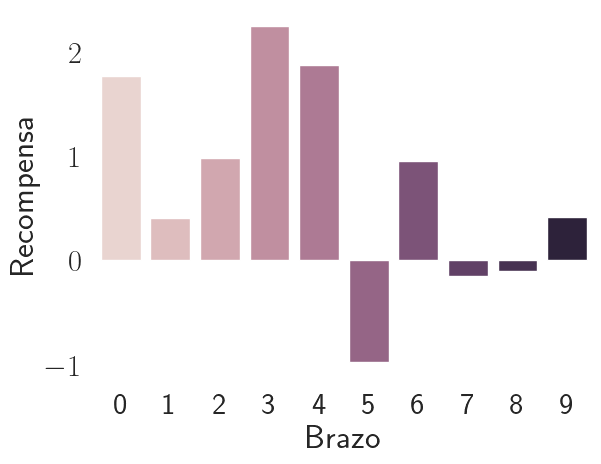
\includegraphics[width=\textwidth]{../img/rewards_sigma_0}
            \caption{$\sigma=0$}
            \label{fig:rewards_0}
        \end{subfigure}
        \begin{subfigure}[H]{0.3\textwidth}
            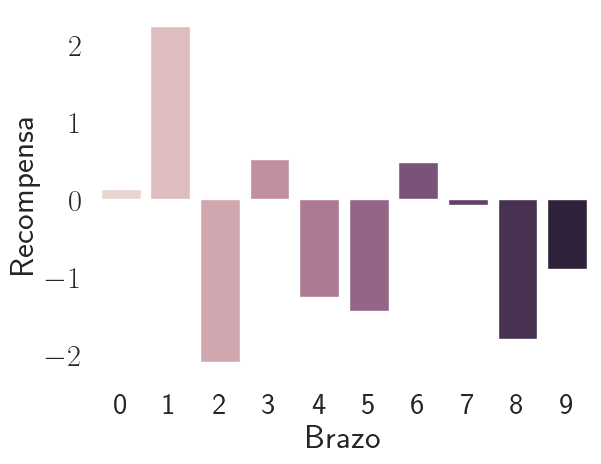
\includegraphics[width=\textwidth]{../img/rewards_sigma_1}
            \caption{$\sigma=1$}
            \label{fig:rewards_1}
        \end{subfigure}
        \begin{subfigure}[H]{0.3\textwidth}
            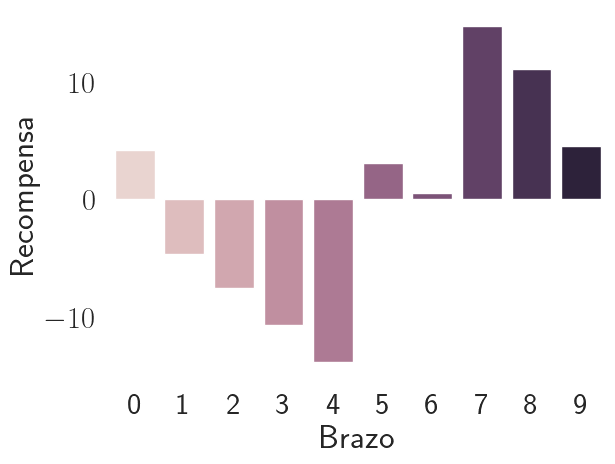
\includegraphics[width=\textwidth]{../img/rewards_sigma_10}
            \caption{$\sigma=10$}
            \label{fig:rewards_10}
        \end{subfigure}
        \caption{Recompensa para cada brazo}
        \label{fig:rewards}
    \end{figure}

    Se aplicó el algoritmo $\varepsilon-greedy$ con distintas combinaciones de $\varepsilon$ y $\sigma$.
    Los resultados de los \textit{Q-valor} de las acciones se muestran en la Figura~\ref{fig:estimations}.

    \begin{figure}[H]
        \centering

        \begin{subfigure}[H]{0.3\textwidth}
            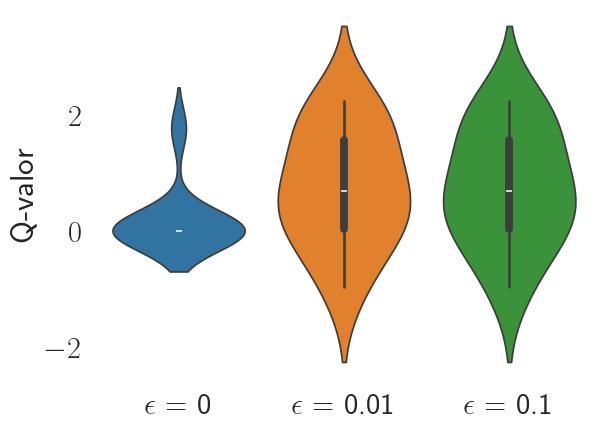
\includegraphics[width=\textwidth]{../img/values_sigma_0}
            \caption{$\sigma=0$}
            \label{fig:estimations_0}
        \end{subfigure}
        \begin{subfigure}[H]{0.3\textwidth}
            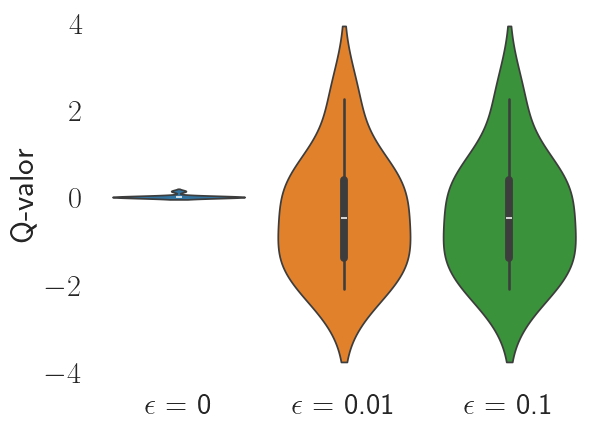
\includegraphics[width=\textwidth]{../img/values_sigma_1}
            \caption{$\sigma=1$}
            \label{fig:estimations_1}
        \end{subfigure}
        \begin{subfigure}[H]{0.3\textwidth}
            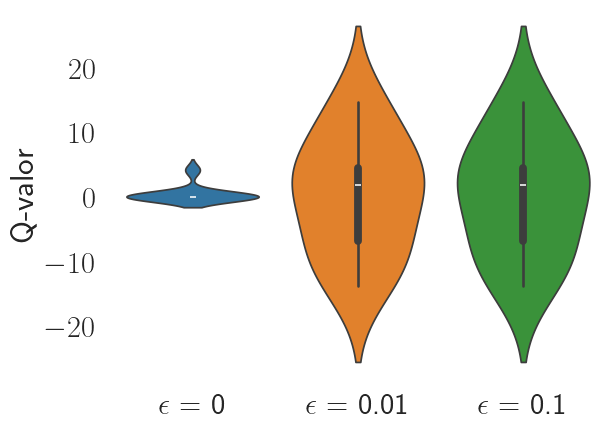
\includegraphics[width=\textwidth]{../img/values_sigma_10}
            \caption{$\sigma=10$}
            \label{fig:estimations_2}
        \end{subfigure}

        \caption{\textit{Q-Valor} de las acciones}
        \label{fig:estimations}
    \end{figure}

    Las figuras~\ref{fig:estimations_0},~\ref{fig:estimations_1} y~\ref{fig:estimations_2} muestran que el Q-valor toma valores cercanos al cero para las acciones en las que $\varepsilon = 0$.
    Esto se debe a que el algoritmo no explora y por lo tanto, no actualiza los valores de las acciones.
    Por otro lado, para $\varepsilon = 0.01$ y $\varepsilon = 0.10$, el algoritmo explora y actualiza los valores de las acciones, lo que permite obtener recompensas mayores.

    La Figura~\ref{fig:arms_selected} muestra el número de veces que se seleccionó cada brazo para los distintos valores de $\varepsilon$ y $\sigma$.

    \begin{figure}[H]
        \centering
        \begin{subfigure}[H]{0.3\textwidth}
            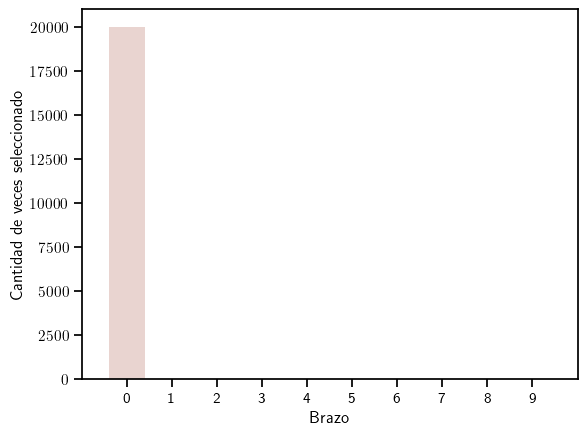
\includegraphics[width=\textwidth]{../img/arm_sigma_0_epsilon_0}
            \caption{$\sigma=0 ,\ \varepsilon=0$}
            \label{fig:arms_selected_0_0}
        \end{subfigure}
        \begin{subfigure}[H]{0.3\textwidth}
            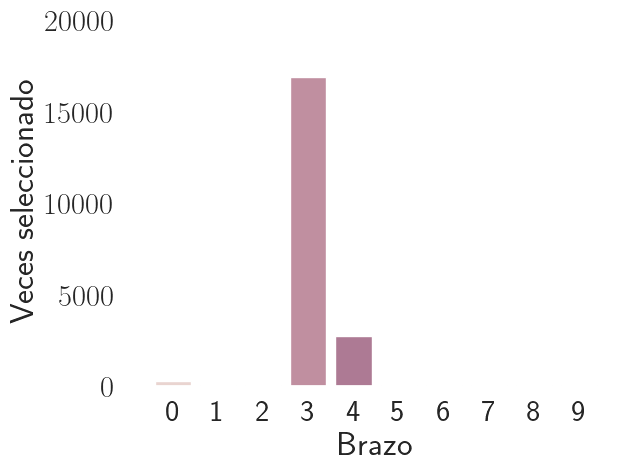
\includegraphics[width=\textwidth]{../img/arm_sigma_0_epsilon_0.01}
            \caption{$\sigma=0 ,\ \varepsilon=0.01$}
            \label{fig:arms_selected_0_0.01}
        \end{subfigure}
        \begin{subfigure}[H]{0.3\textwidth}
            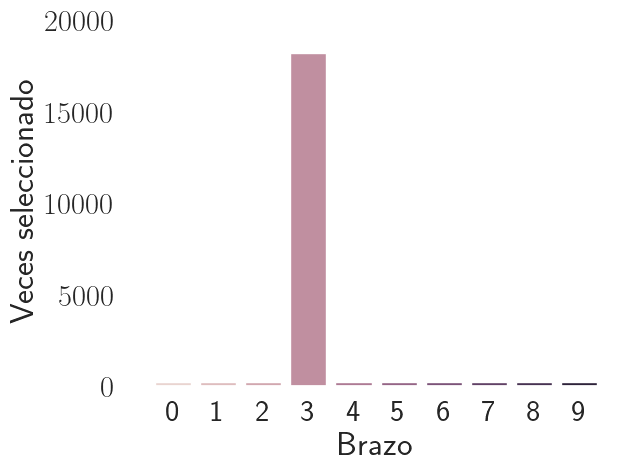
\includegraphics[width=\textwidth]{../img/arm_sigma_0_epsilon_0.1}
            \caption{$\sigma=0 ,\ \varepsilon=0.10$}
            \label{fig:arms_selected_0_0.1}
        \end{subfigure}

        \begin{subfigure}[H]{0.3\textwidth}
            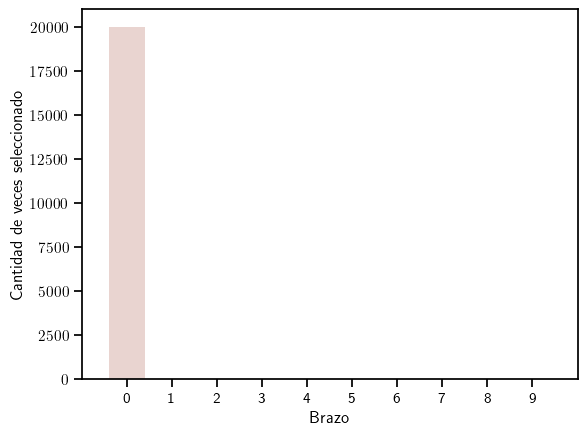
\includegraphics[width=\textwidth]{../img/arm_sigma_1_epsilon_0}
            \caption{$\sigma=1 ,\ \varepsilon=0$}
            \label{fig:arms_selected_1_0}
        \end{subfigure}
        \begin{subfigure}[H]{0.3\textwidth}
            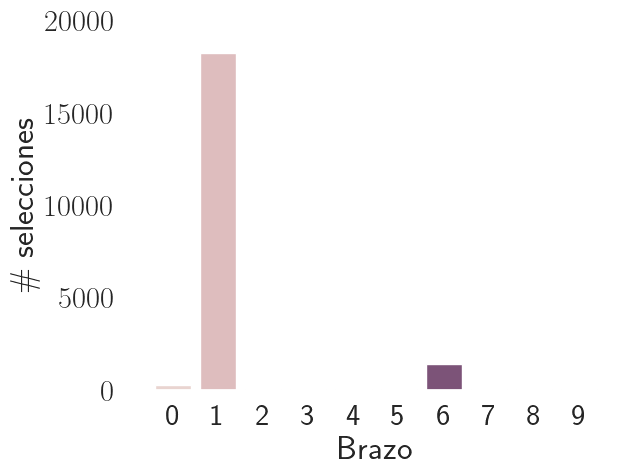
\includegraphics[width=\textwidth]{../img/arm_sigma_1_epsilon_0.01}
            \caption{$\sigma=1 ,\ \varepsilon=0.01$}
            \label{fig:arms_selected_1_0.01}
        \end{subfigure}
        \begin{subfigure}[H]{0.3\textwidth}
            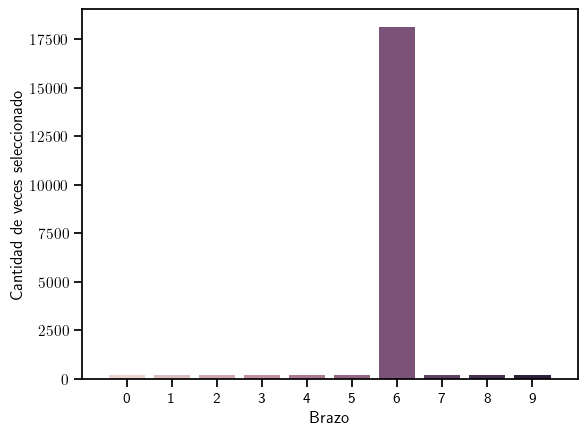
\includegraphics[width=\textwidth]{../img/arm_sigma_1_epsilon_0.1}
            \caption{$\sigma=1 ,\ \varepsilon=0.10$}
            \label{fig:arms_selected_1_0.1}
        \end{subfigure}

        \begin{subfigure}[H]{0.3\textwidth}
            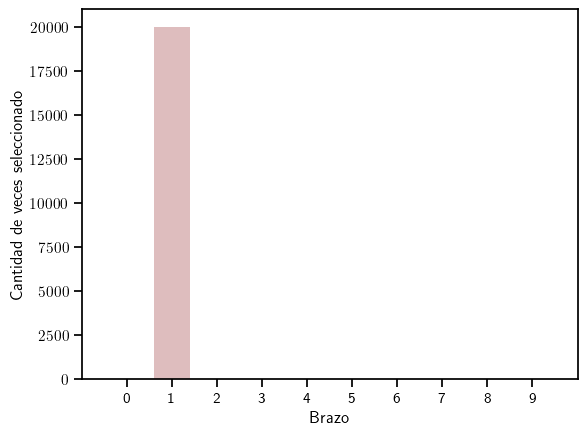
\includegraphics[width=\textwidth]{../img/arm_sigma_10_epsilon_0}
            \caption{$\sigma=10 ,\ \varepsilon=0$}
            \label{fig:arms_selected_10_0}
        \end{subfigure}
        \begin{subfigure}[H]{0.3\textwidth}
            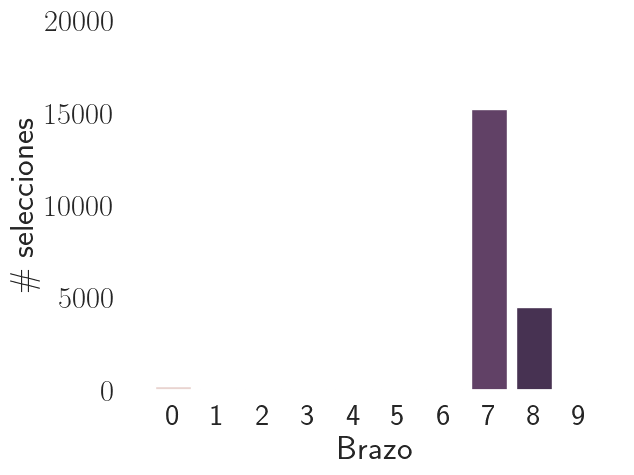
\includegraphics[width=\textwidth]{../img/arm_sigma_10_epsilon_0.01}
            \caption{$\sigma=10 ,\ \varepsilon=0.01$}
            \label{fig:arms_selected_10_0.01}
        \end{subfigure}
        \begin{subfigure}[H]{0.3\textwidth}
            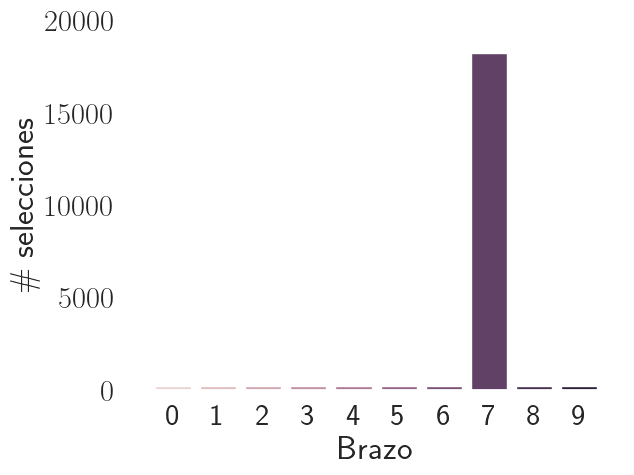
\includegraphics[width=\textwidth]{../img/arm_sigma_10_epsilon_0.1}
            \caption{$\sigma=10 ,\ \varepsilon=0.10$}
            \label{fig:arms_selected_10_0.1}
        \end{subfigure}

        \caption{Número de veces que se seleccionó cada brazo}
        \label{fig:arms_selected}
    \end{figure}

    Finalmente, se analizó la recompensa promedio obtenida en función del número de iteraciones para los distintos valores de $\varepsilon$ y $\sigma$.
    Los resultados se muestran en la Figura~\ref{fig:average_reward}.

    \begin{figure}[H]
        \centering
        \begin{subfigure}[H]{0.3\textwidth}
            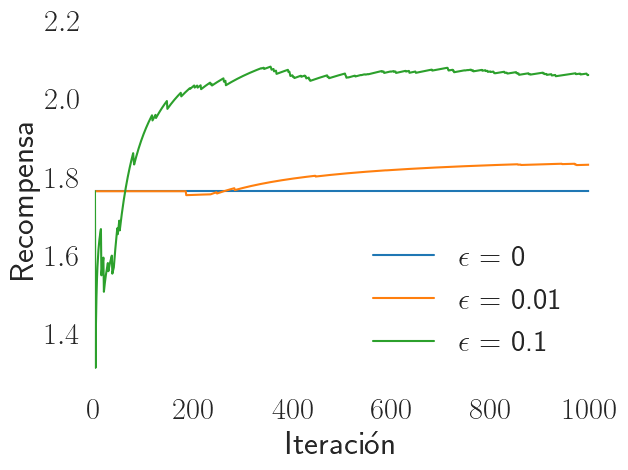
\includegraphics[width=\textwidth]{../img/reward_iteration_sigma_0}
            \caption{$\sigma=0$}
            \label{fig:average_reward_0}
        \end{subfigure}
        \begin{subfigure}[H]{0.3\textwidth}
            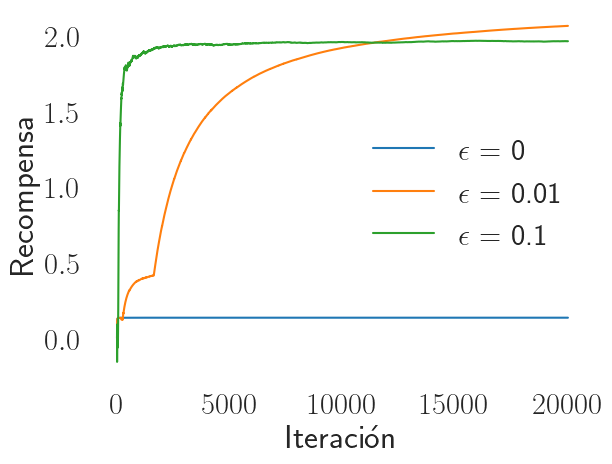
\includegraphics[width=\textwidth]{../img/reward_iteration_sigma_1}
            \caption{$\sigma=1$}
            \label{fig:average_reward_1}
        \end{subfigure}
        \begin{subfigure}[H]{0.3\textwidth}
            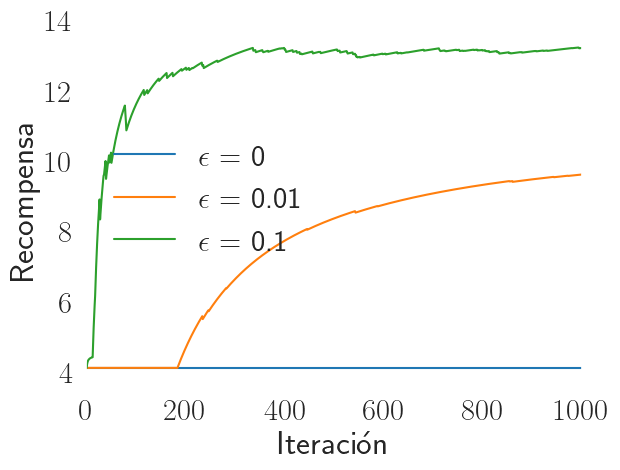
\includegraphics[width=\textwidth]{../img/reward_iteration_sigma_10}
            \caption{$\sigma=10$}
            \label{fig:average_reward_10}
        \end{subfigure}
        \caption{Recompensa promedio obtenida}
        \label{fig:average_reward}
    \end{figure}

    En las figuras~\ref{fig:average_reward_0},~\ref{fig:average_reward_1} y~\ref{fig:average_reward_10} se observa que la recompensa promedio obtenida es cero para todos los valores de $\varepsilon$ y $\sigma$.

    \line(1,0){\textwidth}

    \indent\underline{Ejercicio 6}

    Dada la fórmula adaptativa del valor $Q_{n+1}= Q_n+\alpha\left[R_{n}-Q_{n}\right]$ con $\alpha\in\left(0,1\right]$, demostrar que

    \begin{itemize}
        \item $Q_{n+1}=(1-\alpha)^{n}Q_{n} + \sum_{i=1}^n \alpha(1-\alpha)^{n-i}R_{i}$
        \item $(1-\alpha)+\sum_{i=1}^{n} \alpha(1-\alpha)^{n-i}=1$, es decir, $Q_{n+1}$ es un promedio pesado de $Q_{n},R_1,R_2,\dots,R_n$.
    \end{itemize}

    \indent\underline{Solución:}

    \lipsum[2]

    \line(1,0){\textwidth}

    \indent\underline{Ejercicio 7}

    Demostrar que fórmula adaptativa para calcular el valor $Q_{n+1}=Q_n+\alpha\left[R_n-Q_n\right]$ con  \textit{step-size} $\alpha\in\left(0,1\right]$ constante no verifica las hipótesis del teorema de convergencia y, por lo tanto, no está garantizada su convergencia.

    \indent\underline{Solución:}

    \lipsum[2]

    \line(1,0){\textwidth}

    \indent\underline{Ejercicio 8}

    En la \textit{Figura 2.3} del libro \textit{Sutton\&Barto (2018)}, se observa un \textit{spike} en el paso número 11 cuando se utiliza inicialización optimista.
    De una explicación de este fenómeno.

    \begin{figure}[H]
        \centering
        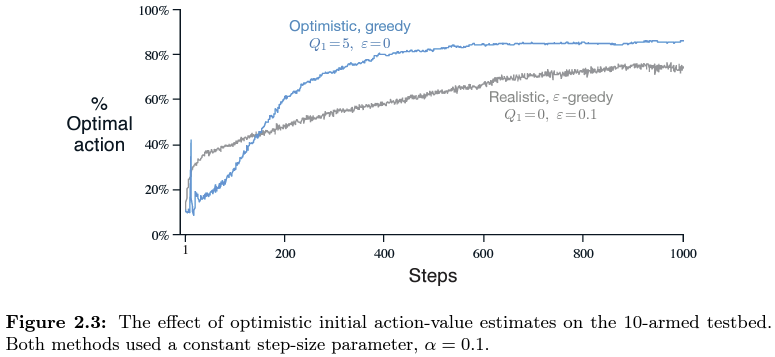
\includegraphics[width=0.5\textwidth]{../img/Figura2_3_SuttonBarto}
        \caption{Figura 2.3 - Sutton\&Barto (2018)}
        \label{fig:fig_2_3}
    \end{figure}

    \indent\underline{Solución:}

    \lipsum[2]

    \line(1,0){\textwidth}

    \indent\underline{Ejercicio 9}

    Demuestre que la función SOFTMAX: $p(a)=\frac{e^{H(a)}}{\sum_{a'=1}^{K} e^{H(a')}}$, define una distribución de probabilidades discreta válida.

    \indent\underline{Solución:}

    \lipsum[2]

    \line(1,0){\textwidth}

    \indent\underline{Ejercicio 10}

    Demostrar que las derivadas de la función SOFTMAX $p(x)$ respecto de sus parámetros $H(a),\ a=1,2,\dots,K$, son iguales a:

    \[
        \frac{\partial p(x)}{\partial H(a)} =
        \begin{cases}
            p(x)(1-p(x))    &\text{si $x = a$} \\
            -p(x)p(a)       &\text{si $x\neq a$}
        \end{cases}
    \]

    \indent\underline{Solución:}

    \lipsum[2]

    \line(1,0){\textwidth}

    \indent\underline{Ejercicio 11}

    Demostrar que la regla de actualización por gradiente ascendente estocástico:

    \[H_{t+1}(a) = H_t (a) + \alpha \frac{\partial E[R_t] }{\partial H_t(a)}\]

    con $E[R_t] = \sum_{x=1}^{K p_t(x)q*(x)}$, puede escribirse de la siguiente manera:

    \[
        H_{t+1}(a) =
        \begin{cases}
            H_t (a) + \alpha (R_t - C)(1-p_t(a))    &\text{si $a = A_t$} \\
            H_t (a) - \alpha (R_t - C)p_t(a)        &\text{si $a \neq A_t$}
        \end{cases}
    \]

    \indent\underline{Solución:}

    \lipsum[5]

    \line(1,0){\textwidth}

    \paragraph{Referencias}\label{sec:references}
    \lipsum[5]

    \paragraph{Apéndice}\label{sec:appendix}

    \lipsum[5]


\end{document}
